\begin{figure}[t]
\centering
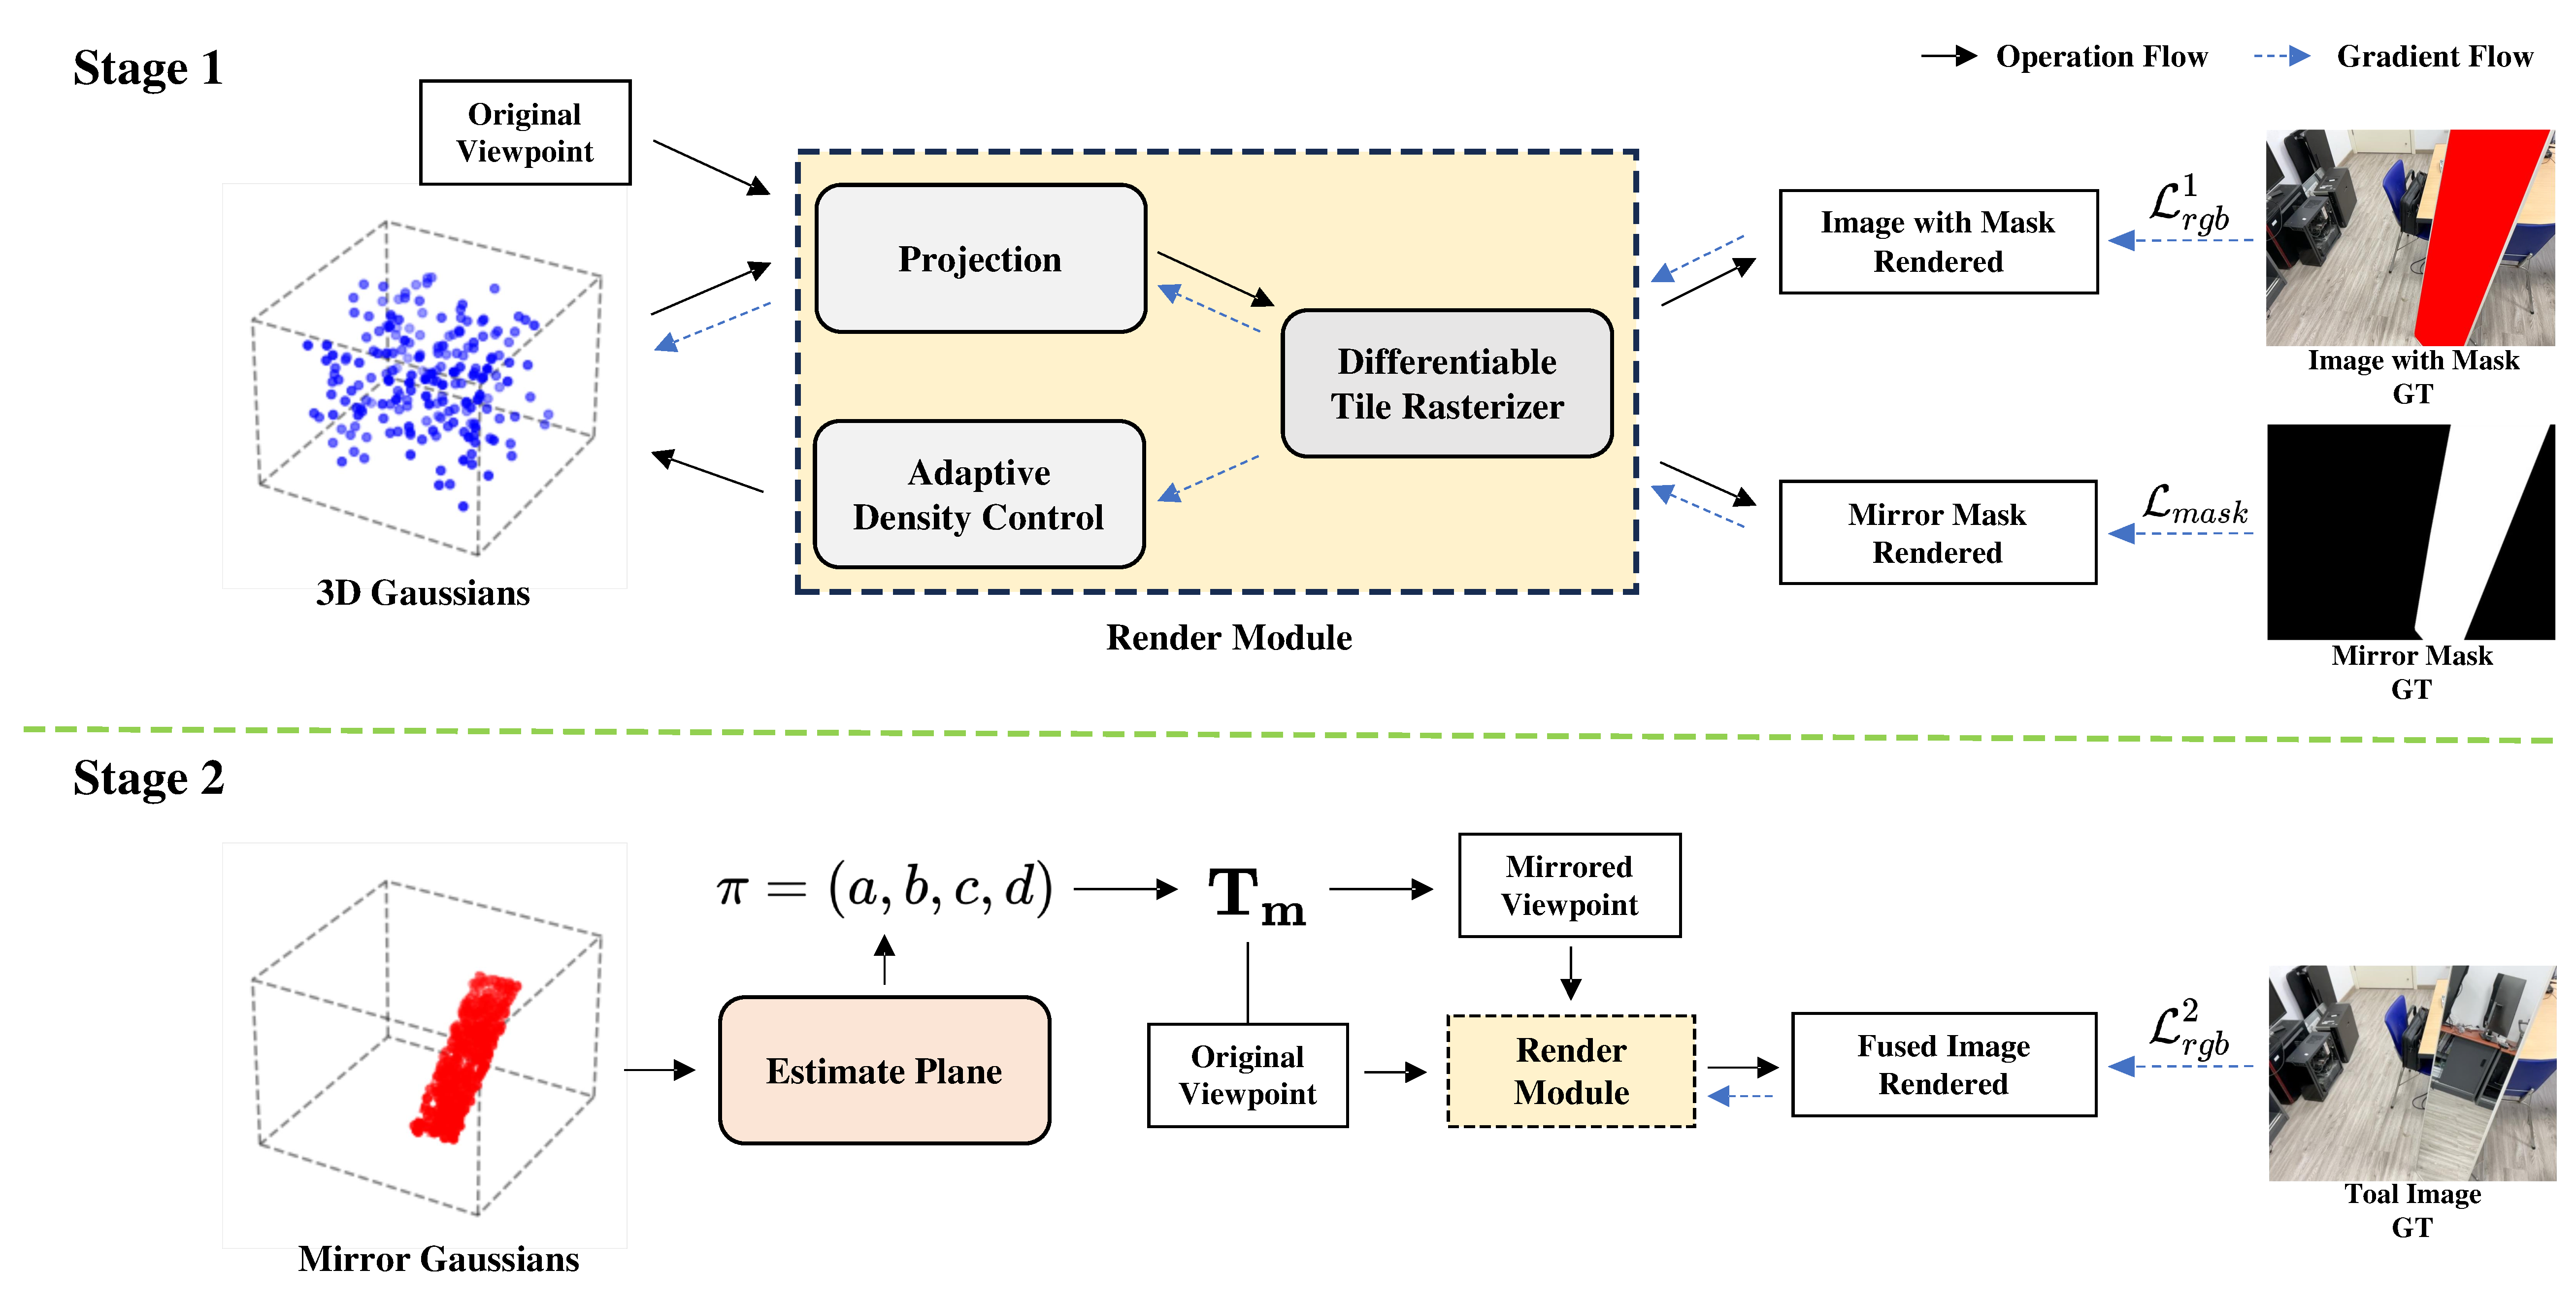
\includegraphics[width=\columnwidth]{file/pipe.pdf}
\caption{\textbf{The illustration of our two-stage training pipeline.} In the \textbf{Stage 1}, we use the mirror mask and view image with mirror content replaced by red to learn the mirror plane and a coarse 3D Gaussian representation of the scene.  In the \textbf{Stage 2},based on the estimated mirror plane, we fuse views from the original and mirrored viewpoints to form the final rendered result, further optimizing the 3D Gaussians.} 
\label{figure:train pipe}
\vspace{-5mm}
\end{figure}
